\white{Pneumatics (May 20, 2024)}
\label{Pneumatics}
\chapterauthor{Caleb Bachmeier}
\info{Caleb Bachmeier}{Pneumatics}{May 20, 2024}
\textbf{Goal}: Explain the VEX V5 Pnuematic system, and how we could use it for our robot this season.
\section*{Overview of VEX V5 Pneumatics}

Pneumatics in the VEX Robotics Competition (VRC) involve the use of compressed air to create mechanical motion. VEX V5 pneumatics systems allow robots to perform various tasks such as lifting, grabbing, or moving objects with precise control. These systems can be particularly useful in achieving tasks quickly and with less motor usage, which can be advantageous given the limited number of motors allowed in VEX competitions.

\section*{Components of a VEX V5 Pneumatics System}

\begin{itemize}
    \item \textbf{Pneumatic Cylinders}: Convert compressed air into linear motion. Available in different sizes and stroke lengths.
    \item \textbf{Solenoid Valves}: Control the flow of air into and out of the cylinders. Available in single-acting and double-acting types.
    \item \textbf{Air Reservoir}: Stores compressed air that powers the pneumatic system.
    \item \textbf{Tubing and Fittings}: Connect the various components, allowing air to flow through the system.
    \item \textbf{Pressure Regulator}: Controls the pressure of the air supplied to the system, ensuring safe and functional limits.
    \item \textbf{Pump}: Manual or electric pump used to initially fill the air reservoir with compressed air.
\end{itemize}
\centering \textbf{}
\begin{figure}[hbt!] % Use [hbt!] to place the figures on the same page
    \begin{minipage}{.5\textwidth}
        \centering
        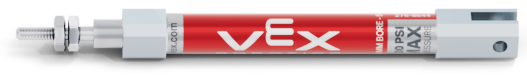
\includegraphics[width=.8\linewidth]{images/Double Action Pneumatic Piston.png}
        \caption{Double Action Cylinder}
        \label{fig:double-action-pneumatic-piston}
    \end{minipage}
    \begin{minipage}{.5\textwidth}
        \centering
        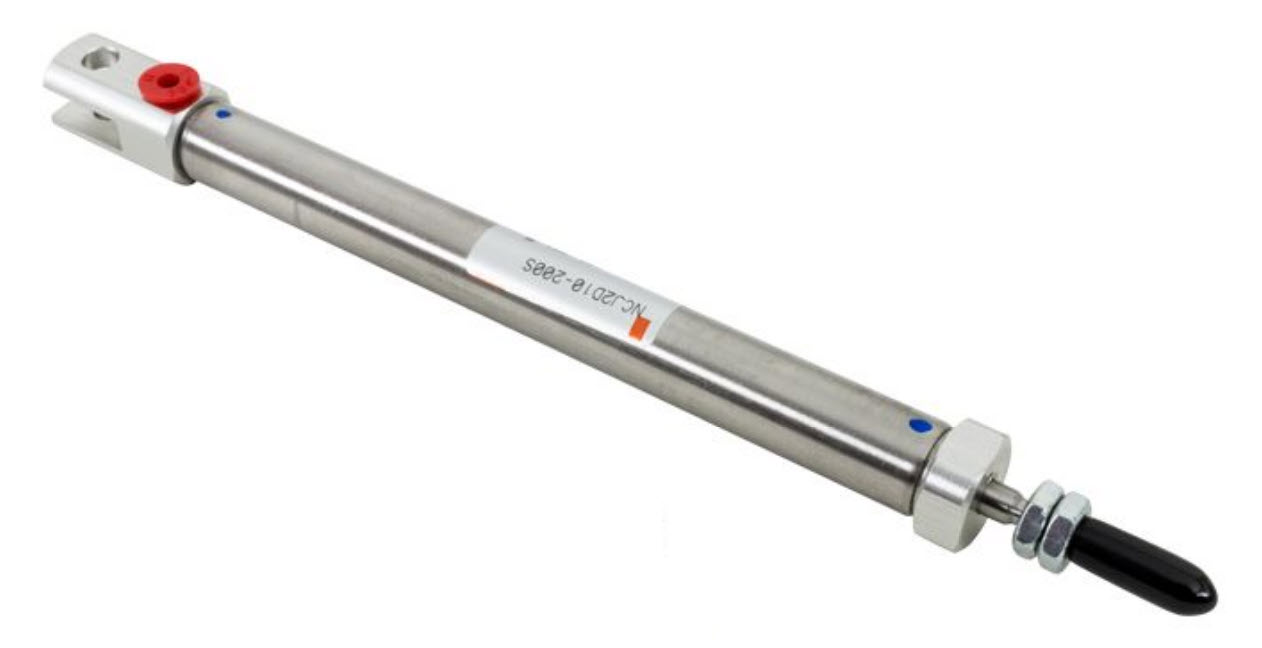
\includegraphics[width=.8\linewidth]{images/Single Action Cylinder.jpg}
        \caption{Single Action Cylinder}
        \label{fig:single-action-cylinder}
    \end{minipage}
    \begin{minipage}{.5\textwidth}
        \centering
        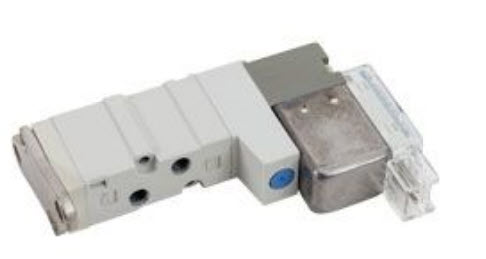
\includegraphics[width=.8\linewidth]{images/Solenoid.jpg}
        \caption{Solenoid}
        \label{fig:solenoid}
    \end{minipage}
    \begin{minipage}{.5\textwidth}
        \centering
        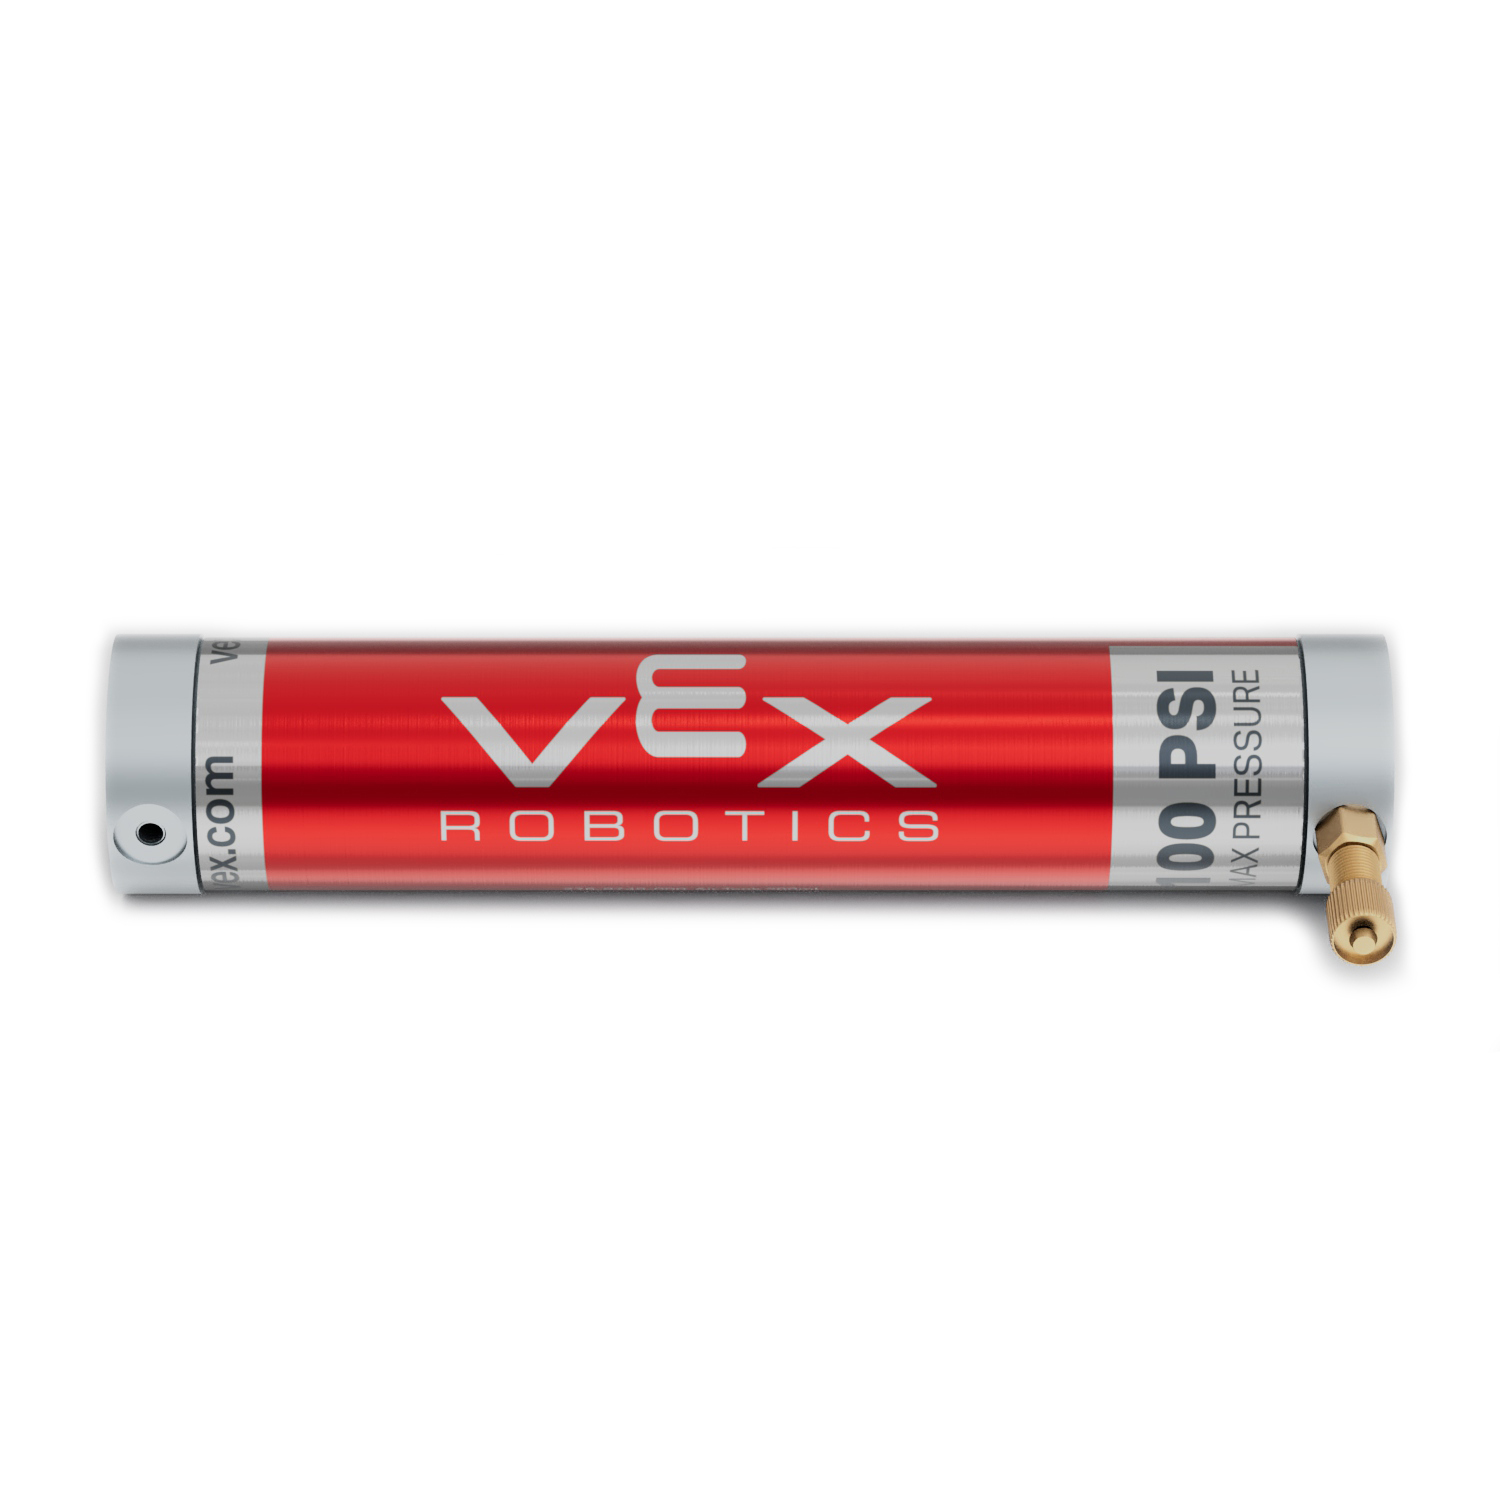
\includegraphics[width=.8\linewidth]{images/Air Resivoir.png}
        \caption{Air Reservoir}
        \label{fig:air-reservoir}
    \end{minipage}
        \begin{minipage}{.5\textwidth}
        \centering
        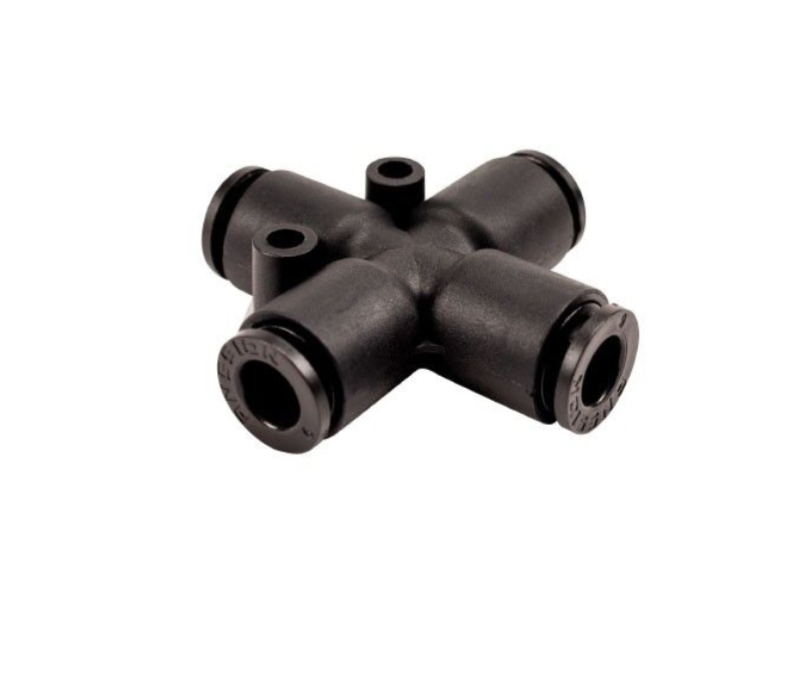
\includegraphics[width=.8\linewidth]{images/Fittings.jpeg}
        \caption{Fittings}
        \label{fig:fittings}
    \end{minipage}
        \begin{minipage}{.5\textwidth}
        \centering
        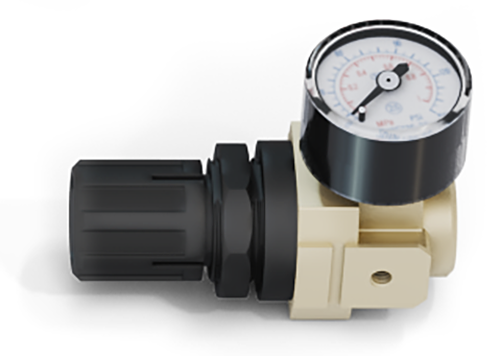
\includegraphics[width=.8\linewidth]{images/Pressure Regulator.png}
        \caption{Pressure Regulator}
        \label{fig:pressure-regulator}
    \end{minipage}
\end{figure}

\pagebreak
\section*{Advantages and Disadvantages of Pneumatics}

\subsection*{Advantages}

\begin{itemize}
    \item \textbf{Quick Actuation}: Provides faster actuation compared to motors, allowing for quicker response times.
    \item \textbf{Strong Force}: Generates significant force, useful for tasks requiring high power, like lifting heavy objects.
    \item \textbf{Efficiency}: Reduces the load on motors, advantageous given the motor limits in VEX competitions.
    \item \textbf{Precision}: Provides precise and repeatable motion, beneficial for tasks requiring accuracy.
    \item \textbf{Motor Maximum}: Pneumatics do not count towards our 88 watt motor limit
\end{itemize}

\subsection*{Disadvantages}

\begin{itemize}
    \item \textbf{Limited Air Supply}: Once the air in the reservoir is depleted, the system requires recharging, limiting usage during matches.
    \item \textbf{Complexity}: Adds complexity to the robot design and requires careful planning and maintenance.
\end{itemize}

\section*{Strategic Use in the 24-25 High Stakes Season}

Effective use of pneumatics could significantly enhance our robot's performance for the 24-25 VEX VRC High Stakes season. Here are some strategic applications:

\subsection*{Claw Mechanism}
Using pneumatic cylinders to operate a claw for grabbing and releasing objects quickly and with high force.

\subsection*{Lifting Mechanism}
Implementing a pneumatic lift to raise and lower objects rapidly, beneficial for stacking tasks or reaching high goals.

\subsection*{Endgame Tasks}
Designing pneumatic mechanisms specifically for endgame tasks that require fast and powerful actuation, such as deploying scoring elements or expanding the robot to control areas.

\subsection*{Multi-Functionality}
Creating mechanisms that can perform multiple functions, such as a single pneumatic system that can both lift and grab, reducing the need for additional motors.

\section*{Example Design: Pneumatic Claw and Lift System}

\subsection*{Claw Design}
Use two double-acting pneumatic cylinders for the claw to provide strong and reliable gripping force. Control the cylinders with solenoid valves, allowing precise control over the opening and closing of the claw.

\subsection*{Lift Design}
Implement a scissor lift or a linear slide mechanism powered by pneumatic cylinders. Use a pressure regulator to ensure the lift operates within safe pressure limits and to control the speed of the lift.

\subsection*{Integration}
Connect the claw and lift to a single air reservoir to save space and weight. Use a manual pump to recharge the reservoir between matches, ensuring the system is always ready for maximum performance.

\subsection*{Control System}
Program the VEX V5 brain to control the solenoid valves based on input from sensors and user commands. Use limit switches or potentiometer to provide feedback on the position of the claw and lift, allowing for precise control.

\section*{Equations}

\subsection*{Equation for Linear Force}
The equation for the ideal linear force generated by a pneumatic cylinder is:
\[
\text{Ideal Linear Force} = \pi \left( \frac{\text{B}_\text{in}}{2} \right)^2
\]
In which:
\begin{itemize}
    \item \textbf{B} is the bore of the pneumatic cylinder (the diameter of the cylinder's internal chamber).
\end{itemize}

This equation calculates the cross-sectional area of the bore, which is then multiplied by the pressure to determine the force exerted by the pneumatic cylinder.

\subsection*{Equation for Volume Reduction per Stroke}
The equation for the volume reduction per stroke of a pneumatic system is:
\[
\Delta V = \left(\frac{\text{B}_\text{in}}{2}\pi \right)^2 \cdot \text{stroke}_\text{in} + \left(\frac{\text{tube cross-section}_\text{in}}{2}\pi \right)^2 \cdot \text{tube length}_\text{in}
\]
In which:
\begin{itemize}
    \item \textbf{B} is the bore of the pneumatic cylinder.
    \item \textbf{Stroke} is the distance the piston travels within the cylinder.
    \item \textbf{Tube Cross-section} is the diameter of the tubing connected to the pneumatic cylinder.
    \item \textbf{Tube Length} is the length of the tubing connected to the pneumatic cylinder.
\end{itemize}

This equation calculates the total volume reduction in the pneumatic system when the piston moves through its stroke. The first term represents the volume change in the cylinder, and the second term represents the volume change in the tubing.

In order to calculate total volume of the system at an given point in time, a basic formula can be derived. By starting with the combined gas law: \[\frac{V_1\cdot P_1}{T_1} = \frac{V_2\cdot P_2}{T_2}\]
\begin{itemize}
    \item \textbf{v} is the volume at a given interval
    \item \textbf{p} is the pressure of the system at a given interval
    \item \textbf{t} is the temperature in degrees kelvin at a given interval
\end{itemize}
In our example, temperature is assumed to be constant, giving the formula: \[V_1\cdot P_1 = V_2\cdot P_2\]
Using algebra to solve for $P_2$... \[P_2 = \frac{V_1\cdot P_1}{V_2}\]
And plugging it into a usable formula for residual computation... \[P_n = \frac{P_{n-1}\cdot V}{V + \Delta V}\]

\subsection*{Real-Time Computation (Added October 15, 2024)}

In order to calculate or air pressure mid match, we need a couple of known variables. 
\begin{itemize}
    \item The total volume of the system $(V)$.
    \item The volume of each section of the system after a solenoid that could be cycled, referred to as $(\Delta V)$.
    \item The initial pressure $(P_1)$ of the pneumatic system (what we set it to at the beginning of the match).
\end{itemize}
While our team could set our pneumatic to any pressure between 0 and 100 (per rule \textless R23\textgreater, clause b: Pneumatic devices may be charged to a maximum of 100 psi.), we do have an experimentally determined minimum of about \(50\text{psi}\). We could calculate a precise minimum based on the force exerted and required by each mechanism, but this is not strictly necessary and is much easier to determine experimentally. It makes sense the most amount of sense to use $100psi$ as our initial \(P_1\) value as per the formulation in the last chapter higher a \(P_1\) provides the most amount of cycles.

%caleb pls fix this. Also, add that it was added in at a later date.

When designing the software for residual pressure computation, I originally came up with three (3) initial solutions. 
\begin{itemize}
    \item Brute force within the \begin{verbatim}
        opcontrol()
    \end{verbatim} loop.
    \item Set a function for volume calculations for each possible action.
    \item Create classes for each type of component that can store volume, subsystems, and the system as a whole.
\end{itemize}
The advantage of using brute force is that it would be quick to implement. However, it would be a solution that would be very loosely held together and almost impossible to modify to fit a separate scenario. Also, any number of edge cases might break it. If we were to make a function for each case we call in the program, it would be faster to implement and cleaner, however, it would not be reproducible. The final option would be to create different classes for each component, subsystem, and system to handle calculations and values. This would take a long time to implement, but it would provide the most modularity out of the three solutions presented. With a few weeks, the best solution that appeared for the criterion and available resources was to develop everything within classes. 
%remember to verbatim the code class and stuff here

\section*{Maintenance and Safety}

\subsection*{Regular Checks}
Regularly check the pneumatic system for leaks, ensuring that all connections are secure and airtight.

\subsection*{Pressure Monitoring}
Continuously monitor the pressure in the reservoir and the system to prevent overpressurization.

\subsection*{Component Inspection}
Regularly inspect pneumatic cylinders, solenoid valves, and tubing for wear and tear, replacing components as needed.

\section*{Conclusion}
By strategically implementing VEX V5 pneumatics, our team can create a highly efficient and powerful robot for the 24-25 High Stakes season. We will focus on leveraging the strengths of pneumatics for tasks that require quick, powerful, and precise motions, and we will ensure that our system is well-maintained and carefully integrated into our overall robot design
\white{Initial Robot Idea (May 21, 2024)}
\label{Initial-Robot-Idea}
\chapterauthor{Ian Smith}
\info{Ian Smith}{Initial Robot Idea}{May 21, 2024}
\section*{Initial Robot Idea}
The first bot idea of the season was originally a conveyor belt-type robot with a floating intake, but after waiting about a week our team had seen numerous robot reveal videos on the Internet of teams executing almost exactly our idea. \blueref{fig:44252A}{Teams like 44252A.} We would like to consider some alternate ideas such as the following: a highly advanced and optimized claw bot, and a robot with a design very similar to \href{https://www.youtube.com/watch?v=HGlivnB0J8U}{this robot by JHAWK} a VEX U team. Now, this robot is obviously a joke and not meant to be taken seriously (it violates SG2 multiple times), but nevertheless it is a good explanation at what we are trying to accomplish. A good claw would be able to add rings to stakes, descore them, and move stakes around. 
\begin{figure}
    \centering
    \includegraphics[width=0.5\linewidth]{images/44252A.jpeg}
    \caption{Team 44252A's Idea}
    \label{fig:44252A}
\end{figure}
\section*{Final Decision} 
After careful consideration and a conference, it was determined that the best idea was to build an inspired but optimized version of \blueref{fig:round-up}{this robot from Round Up}. This was at the time seen as the best idea because it offered a quick reliable scoring mechanism with a reliable descore; being perfectly ideal for competing in skills under ML control.
\begin{figure}[!ht]
    \centering
    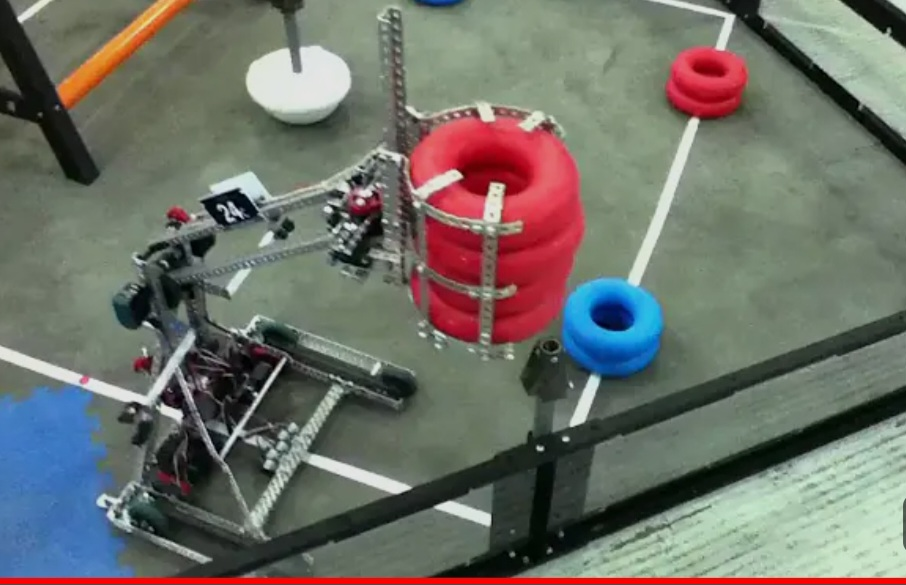
\includegraphics[width=0.5\linewidth]{images/RoundUp.jpeg}
    \caption{Round Up Meta}
    \label{fig:round-up}
\end{figure}
\section*{Design Process}
When designing the bot in fusion, an arc was drawn between the stake and the intake with the center-point of the arc being the location where the pivot would have to be in order to make the arm work. (show a picture of the arc in fusion here) when the pivot was chosen, a c channel was erected to meet the pivot point. From there, gearing and the axle were added along with the 2bar in order to control the length of the pivot of the grabbing mechanism. On the grabbing mechanism itself, a 1:1 ratio was established between the pivot and the central pivoting axle using chains. On the axle itself, lock bars were used to connect the low strength axle to the c channel on the grabbing mechanism rigidly. 
\begin{figure} [h!]
    \centering
    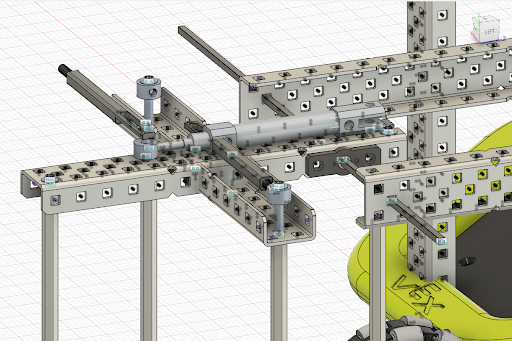
\includegraphics[width=0.5\linewidth]{images/Bot Idea One.png}
    \caption{Mechanism Concept}
    \label{fig:bot-idea-one}
\end{figure} 
\section*{Mechanism Concept}
The concept was that a pneumatic would provide linear force and a separate mechanism would translate the linear force into rotational force which would be able to rotate 90 degrees and force a steel plate under the ring to lock it into place. The only issue: there is not a good space efficient way to translate the force using standard vex parts. The best solution to this problem seemed to be to machine a custom part out of vex parts to accomplish the given task. A part was drawn that would have a slot for the force to be translated in (pinslot mech), and a threaded end on the opposite end of the bar which connected to a shaft collar on the opposite end of the spacing rod.

\section*{Custom Parts Manufacturing}
The following process would be used to make the custom parts:
\begin{itemize}
\item Part off the high strength axle at length
\item Mill the slot on the x axis in order to create the bypass slot on the part
\item Mill the slot on the z axis for the pin screw to sit in
\item Turn down the other side of the part to dimension in order to create a cylinder
\item Cut threads into the turned down cylinder with a die
\item Gently file the part to remove sharp edges
\end{itemize}
 \begin{figure}[h!]
     \centering
     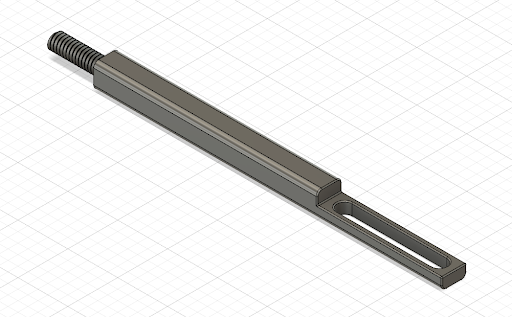
\includegraphics[width=0.5\linewidth]{images/Milled Part.png}
     \caption{Milled Part}
     \label{fig:milled-part}
 \end{figure}
\section*{Design Abandonment}
After drawings were finished, a critical flaw was exposed in the concept: the rings will not be able to bypass the 2bar supports with the constant downward position of the grabbing mechanism. Thus, the design was abandoned with no reasonable solutions to the problem.
\white{Second Bot Idea (May 22, 2024)}
\label{Second-Bot-Idea}
\chapterauthor{Ian Smith}
\info{Ian Smith}{Second Bot Idea}{May 22, 2024}
\section*{Second Robot Idea}

After the failure of the first robot idea, it was determined in a team meeting that the best course of action going forward would be to do the other original idea: an over-engineered clawbot. This concept would be somewhat similar to that last one with a specified pickup area, a stake on a Mogo mechanism, and a claw mechanism that was capable of picking up two rings at the same time  also, this mechanism would be capable of descoring off of the rings, which the last design would not be able to proficiently do.

\section*{Design Considerations}

When going about this idea, {Chase originally came up with the idea of using a pneumatic wrist in order to change position, but it was quickly determined that the binary positions of such a wrist would not provide much benefit. It was then determined that a locked position would be needed on the end of the two bar radius link, and due to motor constraints, the claw would have to be activated pneumatically.
\begin{figure}[h]
    \centering
    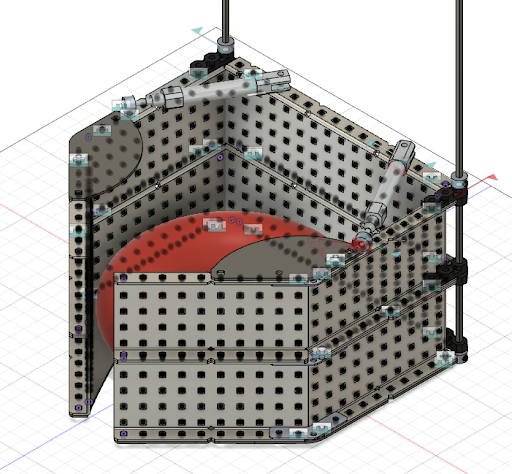
\includegraphics[width=0.5\linewidth]{images/Bot Idea Two.png}
    \caption{Caption}
    \label{fig:bot-idea-two}
\end{figure}
\pagebreak
\section*{CAD Design}
After a general concept was drawn up at practice, I went home and started drawing up some CAD for the idea. When making the CAD, the general idea was to try to use mostly VEX parts for prototyping cases and not use too much laser cut poly-carbonate in the initial design. After carefully considering ring size and the like, it was decided to stack two 10 x 5 aluminum C channels with the 45 degree gusset part. When the jaws were done, the back-plate and pivot for the jaws were built. From there the pneumatics were drawn with a basic motion inspired by wings from over under were used. The last step of the claw was to find a way to hold rings. While it could have been done with steel 1x plating, after consideration it was determined to make the parts out of laser cut poly-carbonate. The parts were drawn up to follow the pattern of the jaws with traditional VEX shapes for aesthetic reasons.

\section*{Design Challenges}

When the idea was about to be conceptualized on the drivetrain, a key flaw was exposed: the bot would not be able to score on the wall stakes. One solution was drawn up to fix this, a pneumatic wrist similar to Chase's original idea, but that was quickly thrown out due to the benefits of a different bot design.

\section*{New Bot Design}

The new bot design was going to be similar to many other robots seen on the internet at the time, but with a 2 bar raisable intake. This design was drawn up by  Connor and heavily inspired by 78A.
